\documentclass[a4paper,12pt]{article}
\usepackage[a4paper, margin=1in]{geometry}
\usepackage[utf8]{inputenc}
\usepackage{graphicx}
\usepackage{xcolor}
\usepackage{braket}
\usepackage{amsmath}
\usepackage{amssymb}
\usepackage[headings]{fancyhdr}
\graphicspath{ {./Figures/} }
\usepackage[sorting=none]{biblatex}
\addbibresource{refs.bib}

\usepackage{hyperref}
\hypersetup{
    colorlinks=true,
    linkcolor=blue,
    urlcolor=cyan,
    citecolor=cyan
}

\newcommand{\mytodo}[1]{\textcolor{red}{TODO: #1}}
\newcommand{\thetas}{\vec{\theta}}
\newcommand{\del}{\partial}
\DeclareMathOperator{\tr}{Tr}
\DeclareMathOperator{\Var}{Var}

\newtheorem{definition}{Definition}
\newtheorem{theorem}{Theorem}



\title{Mutual Unbiased Bases as a Countermeasure to Barren Plateaus}

\author{Ittay Alfassi\footnote{Email: ittay.al@cs.technion.ac.il}}

\begin{document}
\maketitle

\thispagestyle{fancy}
\fancyhead[RO]{Project Supervisor:\\{Prof. Tal Mor}}
\fancyhead[LO]{{Project in Advanced Programming - 236503}\\{Project Report}}

\tableofcontents

\section{Introduction}
Noisy, Intermediate-Scale Quantum (NISQ) computers are quantum computers that are limited in certain ways. They are usually limited in the number of qubits, connectivity between qubits, noise, and maximal circuit depth.
A computational paradigm that utilizes NISQ devices is the paradigm of hybrid quantum-classical algorithms.
Most hybrid algorithms translate a given problem into an optimization problem.
The parameters of the optimization problem control some parametrized quantum state, the problem's cost function is evaluated on the quantum computer, and the optimization steps are performed by the classical computer. These algorithms are called Variational Quantum Algorithms (VQAs)~\cite{Cerezo2021}. \mytodo{Make sure this is accurate!}

While being a leading methodology for the use of quantum computers today, VQAs suffer from several problems. One such problem is the problem of Barren Plateaus~\cite{mcclean_barren_2018}. Informally, barren plateaus imply that over the optimization parameter space, the gradient of the cost function is negligibly small and the optimization process does not how to converge.

This problem affects many  VQAs that employ different types of quantum circuits and classical optimizers (even those that are gradient-free). As the number of qubits and the depth of the quantum circuits increase, this problem worsens exponentially.
Effectively, this means that VQAs will not be able to give an advantage over their classical counterparts in problems that are not small in size.

To address this issue, in this project, I will try and utilize Mutually Unbiased Bases (MUBs), their states, and their properties.
The basic intuition behind this method is that, for any number of qubits, the set of all MUB states spans the entire Hilbert space (with real coefficients).

Thus, inserting them (in some fashion) into the optimization process can allow for an ``exhaustive search'' over the Hilbert space of all states.

Unfortunately, this method did not succeed. However, I will detail the different aspects of this approach, the experiments implemented, the conclusions I reached, and possible methods to still utilize the idea of MUB states in VQAs.

This project is mainly based on the work of Arrasmith et al.~\cite{arrasmith_effect_2021}.


\section{Preliminaries}

\subsection{Variational Quantum Algorithms}
A Variational Quantum Algorithm is an algorithm that takes some computational problem and solves it by hybrid classical-quantum optimization.
VQAs are comprised of several elements: The quantum circuit, the cost function, and the optimizer.

\begin{enumerate}
    \item \textbf{The Quantum Circuit.} Every VQA problem uses a quantum circuit with some parametric values.
    Its structure can be generally written as the following:
    \begin{equation}
        U(\thetas) = \prod_{l=1}^{L} U_l(\theta_l) W_l
    \end{equation}
    Where $U_l(\theta_l) = \exp(-i\theta_l V_l)$, $V_l$ is a Hermitian operator (thus $U_l$ is a unitary operator), and $W_l$ is a generic unitary operator that does not depend on any angle $\theta_l$.
    
    In some VQAs, an \textbf{initial state} $\ket{\psi_0}$ is also a part of the algorithm, and it is related to the quantum circuit.

    The term \emph{ansatz} (German for ``approach''/``attempt'') is used in literature to either describe the initial state $\ket{\psi_0}$, the parametric circuit $U(\thetas)$, or the application of the parametric circuit to the initial state $\ket{\psi(\thetas)} = U(\thetas)\ket{\psi_0}$.
    In this project, I will use the term ansatz to refer to the parametric quantum circuit.

    Ansatzes\footnote{The correct plural form in German is Ansaetze.} can either be problem-specific or problem-agnostic.

    A problem-specific ansatz is tailored to the problem solved by the VQE using a-priori knowledge of the structure of the problem. Through this tailoring, there is a better chance that the circuit can reach values that are optimal for the problem at hand. When using a problem-specific ansatz, the initial state is usually also tailored according to the same information.
    
    A problem-agnostic ansatz is not tailored to the problem specifically and can be used with no relevant information. It is usually comprised of repeated layers of quantum gates. Each layer is comprised of quantum gates that are usually easy to implement directly on quantum hardware, in contrast to problem-specific ansatzes. Problem-agnostic ansatzes are usually called ``hardware-efficient'' for this reason.
    In this project, I focused on using hardware-efficient ansatzes.
    
    \item \textbf{The Cost Function.} The cost function $C(\thetas)$ defines the goal of the VQA. It is defined as a function from the parameters of the ansatz to the real numbers.
    The goal of the VQA is to find
    \begin{equation}
        \thetas^* = \arg\min_{\thetas} C(\thetas)
    \end{equation}

    The cost function always depends on the ansatz, some Hermitian operators, and some initial states.
    Generally, it can be written as
    \begin{equation} \label{eqn:general_cost}
        C(\thetas) = \sum_k f_k(\tr[O_k U(\thetas) \rho_k U^\dagger(\thetas)])
    \end{equation} 
    Where $\{f_k\}$ is a set of functions, $\{O_k\}$ is a set of operators, and $\{\rho_k\}$ is a set of input states.
    
    The trademark of VQAs is that they use a quantum computer to estimate the cost function $C(\thetas)$ (or its derivatives) while leveraging the power of classical optimizers to train the parameters $\thetas$.
    
    \item \textbf{The Optimizer.} While not necessarily dependent on the problem the VQA is trying to solve, the classical optimizer is an important part of the algorithm.
    The optimizer is run on a classical computer, and performs an iterative process: it uses data on the current parameters of the cost function to calculate their value in the next iteration. More details can be found in subsection~\ref{subsec:optimizers}.
\end{enumerate}


\subsubsection{Example: Variational Quantum Eigensolver}
One of the earliest examples of a VQA is the VQE algorithm, proposed by Peruzzo et al.~\cite{peruzzo_variational_2014}. In this algorithm, The goal is to find the lowest eigenvalue of some Hamiltonian $H$.
The cost function is straightforwardly defined as the expectation value of the parametric state over the Hamiltonian:

\begin{equation}
    C(\thetas) = \bra{\psi(\thetas)} H \ket{\psi(\thetas)} = \bra{\psi_0} U^\dagger(\thetas) H U(\thetas) \ket{\psi_0}
\end{equation}

In case $H$ is a molecular Hamiltonian (converted to a qubit Hamiltonian using an appropriate transformation), a problem-specific ansatz can be used. One such option is the Unitary Coupled-Cluster (UCC) ansatz, together with the Hartree-Fock state as the initial state.

Of course, a hardware-efficient ansatz can be used for any structure of $H$.

\subsubsection{Example: Variational Quantum Compiling}
A different example of a VQA is the problem of Variational Quantum Compiling (VQC), initially defined by Khatri et al.~\cite{khatri_quantum-assisted_2019} as Quantum-Assisted Quantum Compiling (QAQC).

In VQC, the input of the problem is a general $n$-qubit unitary operation $V$.\footnote{In the Khatri paper, the target unitary is denoted as $U$, while the ansatz is denoted $V$. I switched the notations to stay consistent with the rest of the examples and papers.} The goal of the algorithm is to control the parameters of a parametric quantum circuit $U(\thetas)$ so its behavior will be similar to that of $V$.

Formally, there are two possible goals: either that $U(\thetas)$ and $V$ will perform the same operation on all states, or that $U(\thetas)$ and $V$ will perform the same operation on a specific input state.
In this project, I will use the latter as the problem definition. Thus, we wish that $V\ket{\vec{0}} = U(\thetas)\ket{\vec{0}}$.

There are two different cost functions presented in~\cite{khatri_quantum-assisted_2019}.
The first is straightforward and is defined by

\begin{equation}
    C^{\textrm{global}} = 1 - \left|\bra{\vec{0}}UV^\dagger\ket{\vec{0}}\right|^2
\end{equation}

Another cost function, called the local cost function, is defined by 

\begin{equation}
    C^{\textrm{local}} = 1 - \frac{1}{n} \sum_{j=1}^{n} p_0^{(j)}
\end{equation}

where
\begin{equation} \label{eqn:local_vqc_cost}
    p_0^{(j)} = \tr[({\ket{0}\bra{0}}_j \otimes I) U^\dagger V \ket{\vec{0}}\bra{\vec{0}} V^\dagger U]
\end{equation}
and ${\ket{0}\bra{0}}_j \otimes I$ is the tensor product of the matrix $\ket{0}\bra{0}$ in the jth term and identity matrices in all other terms.
The operational meaning of $p_0^{(j)}$ is the probability to obtain the zero measurement outcome on qubit $j$ for the state $U^\dagger V\ket{\vec{0}}$.

it is proven in~\cite{sharma_noise_2020} that

\begin{equation}
    C^{\textrm{local}} \leq C^{\textrm{global}} \leq nC^{\textrm{local}}
\end{equation} 

However, $C^\textrm{global}$ suffers from a provably vanishing gradient as $n$ increases, while $C^\textrm{local}$ does not. Thus, we will use $C^\textrm{local}$ or a linear combination of both costs in our experiments.

\subsection{Optimizers for Variational Quantum Algorithms} \label{subsec:optimizers}
Classical optimizers perform the task of finding a (hopefully global) extremum of some scalar function.
An optimizer for a function $F$ needs to find the vector $\thetas \in S$ with $S \subseteq \mathbb{R}^n$ that gives a minimal or maximal value for $F$. In this project, we will only use optimizers for the minimization of cost functions.

In each step, an optimizer is given a point in the parameter space of the cost function $\thetas_{i}$, and is tasked with finding a new guess for parameter values $\thetas_{i+1}$, which hopefully has a lower cost value.

The optimizer can either use the value of the cost function, its partial derivative (its gradient vector), or its second partial derivatives (its Hessian matrix).

Methods that use the second derivative are often called Newton methods (as Newton's method uses the second derivative). Methods that use \emph{approximations} of the first and second derivative are called Quasi-Newton methods.
Methods that use the first derivative are called Gradient-Based methods. Methods that do not use the derivative at all are called Gradient-Free methods.

In this project, I focused on two gradient-free optimizers: the Powell optimizer and the COBYLA optimizer.

\subsubsection{Powell}
The Powell algorithm~\cite{Powell1964} is a popular gradient-free optimizer that uses sequential line searches (optimizations over lines in the parameter space).

This method starts with some input set of search vectors $V = \{\vec{v}_i\}$, which are usually chosen to be the coordinate vectors in the parameter space. Each vector defines a search direction (both the direction of the vector and its negation).

Searching along each of those directions in sequence, this method looks for the displacement $\{a_i\}$ along each direction that would minimize the cost when only varying parameters along the current direction.
If bounds to the parameter space are specified, the minimization will be under said bounds. If bounds are not provided, then an unbounded line search will be used.
Finding the displacements in each direction is done by some univariate gradient-free optimizer.
Two common options for such an optimizer are Brent's parabolic interpolation method and the Golden-section search method, but their choice is independent of the general Powell method.

After sweeping through all of the search vectors, two updates are made:
First, the current parameters are updated by the rule:
\begin{equation}
    \thetas_{i+1} = \thetas_{i} + \sum_i a_i \vec{v}_i
\end{equation}
Second, the search vector $\vec{v}_j$ that corresponds to the greatest displacement, $a_j = \max(a_i)$ is replaced with
\begin{equation}
    \vec{v_j} \to \sum_i a_i \vec{v}_i.
\end{equation}

The algorithm iterates an arbitrary number of times until no significant improvement to the value of the cost function is made.


\subsubsection{COBYLA}
Constrained Optimization BY Linear Approximation (COBYLA) is a gradient-free numerical optimization method, invented by Powell~\cite{Powell1994,powell_view_2007} (although it is different from the Powell optimization method).

The method tries to optimize a function $F(\thetas)$ according to a set of constraints $\{c_i(\thetas)\}$.

At each iteration, the method has $m+1$ points $\{\thetas_i\}_{i=0}^m$ in the parameter space that are sorted by a combination of the function's value on them and the penalties that the constraints imply on them.
The said sorting function is of the form
\begin{equation}
    \Phi(\thetas) = F(\thetas) + \mu[ \max\{-c_i(\thetas) : i=1,2,\dots,m \} ]_+, \thetas \in \mathbb{R}^n
\end{equation}
For a value $\mu$ that is automatically controlled by the method and the subscript + signifying that 0 is taken in case the value of the expression is negative.
Thus, our points are sorted as $\Phi(\thetas_0) < \Phi(\thetas_1) < \dots < \Phi(\thetas_m)$.

In addition, there is a ``trust region'' with a radius $\rho>0$. The method uses the $m+1$ points as the vertices of a simplex (an $m$-dimensional generalization of a triangle).
The values of the cost function in these vertices are used for interpolation to a unique linear polynomial $\hat{F}(\thetas)$, and the values of the constraint functions in these vertices are used for interpolation to unique linear constraints $\{\hat{c}_i\}$
The method then continues by minimizing $\hat{F}(\thetas)$, which is in the trust region --- that is, $\frac{\rho}{2} \leq \|\thetas - \thetas_0\| \leq \rho$, under the approximated constraints $\{\hat{c}_i\}$.

In case there is no point in the trust region in which all approximated constraints are satisfied, $\thetas$ is defined by minimizing the greatest of the constraint violations subject to the trust region bound.

The newly calculated point is added to the set of points, and some other point is removed.
The choice of the point to be removed is governed mainly by avoiding the degenerate situation where the volume of the simplex collapses to zero, as in that case, only a subspace of the parameter space is reachable.

When the improvements are insufficient, the value of $\rho$ is reduced, until some lower bound, which specifies the termination of the method, is reached.

This explanation of the method is incomplete, and only describes the general principle behind the optimization. In addition, different specifications by Powell (for example, \cite{Powell1994} and \cite{powell_view_2007}) define certain requirements and symbols differently, such as using $\Phi$ or $F$ for the sorting of vertices, the use of $\mu$, and the use of $\rho$ as the trust radius or as a lower bound for it.
Certain technical details and special steps in the method are also omitted and can be found in Section 2 of~\cite{Powell1994}.


\section{Barren Plateaus} \label{sec:bps}
Informally, a barren plateau is a large section of the parameter space in which the value of the cost function $C$ is ``flat'', and has no apparent direction in which to move in order to reach a minimum point. The term was first coined by McClean et al. in~\cite{mcclean_barren_2018}.

When considering a cost function with 2 parameters, this definition coincides with its geometrical intuition. The plane defined by $\{(\theta_1, \theta_2, C(\theta_1, \theta_2)) | (\theta_1, \theta_2) \in \mathbb{R}^2\}$ will have large, flat sections, in which the ``dips'' that represent minima are not indicated by a slope around them (other than a very small neighborhood of the minimum). Such an example can be seen in Figure~\ref{fig:bp}.

\begin{figure}[h]
    \centering
    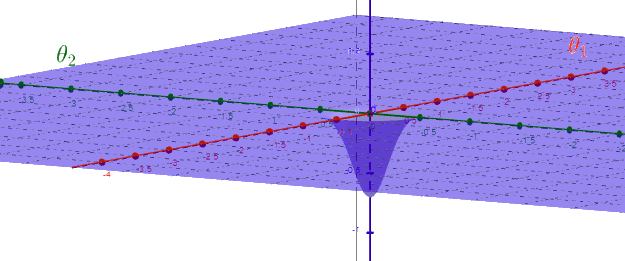
\includegraphics[scale=0.5]{bp_3d.png}
    \caption{A barren plateau in an inverted bi-variate Gaussian with a small variance.}
    \label{fig:bp}
\end{figure}

This is formally defined by the expectation value and variance of the partial derivatives.
As defined in \cite{arrasmith_effect_2021}:

\begin{definition} \label{def:bp}
    Consider the cost function defined in Eq.~(\ref{eqn:general_cost}). This cost exhibits a barren plateau if, for all $\theta_\mu \in \thetas$, the expectation value of the cost function partial derivative
    $\del C / \del\theta_\mu = \del_\mu C(\thetas)$
    is
    $E_{\thetas}[\del_\mu C(\thetas)] = 0$
    and its variance vanishes exponentially with the number of qubits n as 
    \begin{equation} \label{eqn:vanishing}
        \Var_{\thetas}[\del_\mu C(\thetas)] \leq F(n) \textrm{,   with   }F(n) \in O\left(\frac{1}{b^n}\right)
    \end{equation}
    for some $b > 1$. As indicated, the expectation values are taken over the parameters $\thetas$.
\end{definition}

\subsection{Ansatzes and Functions Affected By Barren Plateaus}
Papers in the field of barren plateaus have shown that many types of cost functions exhibit barren plateaus.

The original work by McClean et al.~\cite{mcclean_barren_2018} shows that cost functions of the form in Eq. (\ref{eqn:general_cost}) that use random quantum circuits of polynomial depth and exhibit a property known as a \emph{2-design} suffer from barren plateaus.
The definition of a 2-design is beyond the mathematical scope of this project.

However, the work of Arrasmith et al.~\cite{arrasmith_effect_2021} notes that hardware-efficient layered ansatzes are approximate 2-designs (although they did not show this result themselves).
As such, cost functions that use these ansatzes suffer from barren plateaus when the number of layers scales linearly with the number of qubits.

Another paper, by Cerezo et al.~\cite{cerezo_cost_2021}, shows that if the cost function makes use of global operators, barren plateaus will be encountered in \emph{any} circuit depth.
For this reason, it is preferable to use the local cost function in VQC problems and not the global cost function.
% A paper by Wang et al.~\cite{wang_noise-induced_2021}

\subsubsection{Barren Plateaus in VQC}
In section 4 of Arrasmith~\cite{arrasmith_effect_2021}, it is shown that even a fairly simple VQC problem suffers from barren plateaus.

The specific problem shown in the paper is concerned with the trivial target unitary $V = I$.
Thus, we are trying to optimize the parameters of a parametric quantum circuit $U(\thetas)$ such that $U(\thetas)\ket{\vec{0}} = I\ket{\vec{0}} = \ket{\vec{0}}$.

The quantum circuit used is a layered hardware-efficient ansatz.
Each layer is defined by the following structure:
\begin{itemize}
    \item A general unitary single-qubit rotation gate $U(\theta_1, \theta_2, \theta_3)$ gate is applied to each qubit.
    \item A layer of Control-NOT gates is applied between even pairs of qubits (that is, even indices act as controls and odd indices act as targets).
    \item Another layer of general unitary single-qubit rotations is applied.
    \item A layer of Control-NOT gates is applied between odd pairs of qubits (odd indices act as controls and even indices act as targets).
\end{itemize}
A sketch of a single layer of the circuit can be seen in Figure~\ref{fig:layer}.

The cost function used is the local VQC cost function, as shown in Eq. (\ref{eqn:local_vqc_cost}).
Arrasmith~\cite{arrasmith_effect_2021} claims that when the number of layers scales linearly with the number of qubits, this problem instance suffers from barren plateaus.

\begin{figure}[h]
    \centering
    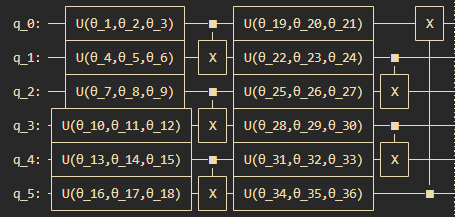
\includegraphics{arrasmith_layer.png}
    \caption{A single layer of the hardware-efficient ansatz used in the project, as designed in Qiskit.}
    \label{fig:layer}
\end{figure}

\subsection{Barren Plateaus in Gradient-Free Optimization}
Seeing as the definition of barren plateaus only discusses the partial derivatives of the cost function, one might assume that using gradient-free optimizers solves this issue.
However, the main result of Arrasmith shows that this is incorrect.

The following theorem is shown in~\cite{arrasmith_effect_2021}:

\begin{theorem}
    Consider the cost function of Eq.~(\ref{eqn:general_cost}). Let ${\thetas}_A$ and $\thetas_B$ be two randomly chosen points in parameter space.
    Without loss of generality we assume that $\thetas_B = \thetas_A + L\hat{l}$ for random $L$ and $\hat{l}$ so that $E_{\thetas_A, \thetas_B}[\dots] = E_{\thetas_A, L, \hat{l}}[\dots]$.
    If the cost exhibits a barren plateau according to Definition~\ref{def:bp}, then the expectation value of the difference $\Delta C = C(\thetas_B) - C(\thetas_A)$ is $E_{\thetas_A, L, \hat{l}}[\Delta C] = 0$, and the variance is exponentially vanishing with n as 
    \begin{equation}
        \Var_{\thetas_A,L,\hat{l}}[\Delta C] \leq \hat{G}(n)
    \end{equation}
    with
    \begin{equation}
        \hat{G}(n) = m^2 \bar{L}^2 F(n)\textrm{,    and     } \hat{G}(n) \in \tilde{O}\left(\frac{1}{b^n}\right).
    \end{equation}
    for some $b>1$. Here m is the dimension of the parameter space, $F(n)$ was defined in (\ref{eqn:vanishing}), and
    \begin{equation}
        \bar{L} = E_{L,\hat(l)}[L]
    \end{equation}
    is the average distance between any two points in parameter space.
\end{theorem}

The effective meaning of this theorem is that the difference in the cost function between different points in the parameter space is exponentially vanishing in $n$.
Thus, even though gradient-free optimizers do not use derivatives, they are still affected --- Their main tool for decision-making, which is the difference in the values of the function, gives almost no information.

\section{Mutually Unbiased Bases}

\subsection{Generation of Mutually Unbiased Bases}

\subsection{MUB States as an Exhaustive Search}


\section{MUB Utilization Techniques}

\subsection{Using All MUB states}

\subsection{Sampling $k$ MUB states}

\subsection{``Half-MUB'' states}


\section{Experiments}

\subsection{Control Group: Random Initialization Vectors}

\subsection{Experiment 1: Reproducing the Arrasmith Barren Plateau}

\subsection{Experiment 2: 3 qubits and $n$ layers}

\subsection{Experiment 3: $n$ qubits and $n$ layers}

\section{Discussion}

\printbibliography
\end{document}
